%!TEX program = xelatex

\documentclass[compress]{beamer}
%--------------------------------------------------------------------------
% Common packages
%--------------------------------------------------------------------------
\usepackage[english]{babel}
\usepackage{pgfpages} % required for notes on second screen
\usepackage{graphicx}

\usepackage{multicol}

\usepackage{tabularx,ragged2e}
\usepackage{booktabs}


%--------------------------------------------------------------------------
% Load theme
%--------------------------------------------------------------------------
\usetheme{hri}

\usepackage{dtklogos} % must be loaded after theme
\usepackage{tikz}
\usetikzlibrary{fpu,calc,fit,mindmap,backgrounds,positioning}

\graphicspath{{figs/}}

\setbeamercolor{refToContribCol}{bg=hriSec1Comp,fg=white}
\setbeamercolor{highlightCol}{bg=hriSec3,fg=white}

\newcommand{\refToContrib}[1]{%
    \begin{beamercolorbox}[wd=\linewidth,ht=2ex,dp=0.7ex]{refToContribCol}%
    \hspace{0.5em}$\hookrightarrow$ #1%
    \end{beamercolorbox}%
}%
\newcommand{\highlight}[1]{%
    \begin{beamercolorbox}[wd=\linewidth,dp=0.7ex]{highlightCol}%
    #1%
    \end{beamercolorbox}%
}%

\newsavebox{\som}
\savebox{\som}{%
    \begin{tikzpicture}[
        input/.style={draw,circle,inner sep=0pt,minimum size=0.25cm}
    ]
        \newcounter{colour}
        \setcounter{colour}{0}
        \foreach \x in {-3, -2, ..., 3}
        \foreach \y in {3, 2, ..., -3}{
            %\node[draw, circle, shading=sphere] at ({(\x + 0.4*\y)/2.2}, {\y/4}) {};
            \pgfmathsetcounter{colour}{((sin(deg(\x)) * sin(deg(\y)))+1)*50}
            %\shade[ball color=green!\thecolour!red] ({(\x + 0.4*\y)/2.2}, {\y/4}) circle (.2cm);
            \node[input, fill=hriSec2!\thecolour!hriSec3] at ({(\x + 0.4*\y)/2.2}, {\y/4}) {};
        };
    \end{tikzpicture}%
}

%--------------------------------------------------------------------------
% General presentation settings
%--------------------------------------------------------------------------
\title{Computational Structures}
\subtitle{Q4 -- How the requirements for social interaction would inform your
choice of the fundamental computational structures of the architecture (e.g.
symbolic, sub-symbolic, hybrid, ...)?}
\date{}
\author{}
\institute{\includegraphics[height=15mm]{plymouth-logo}}
%\\Centre for Robotics \& Neural
%Systems\\{\Medium Plymouth University}}

%--------------------------------------------------------------------------
% Notes settings
%--------------------------------------------------------------------------
%\setbeameroption{show notes on second screen}

\begin{document}

\maketitle

\begin{frame}{General perspectives}

    \highlight{\centering Support modelling (human) social cognition\\\scriptsize(application to robots nice to have)}

        \vspace{2em}
        or...\\
        \vspace{1em}

        \highlight{\centering Support thinking about robot programming \\in term of socio-cognitive skills}

\end{frame}
%{
%\paper{Lemaignan et al., {\Medium Towards Grounding Human-Robot Interaction}, 2012}

\begin{frame}{Symbolic architectures for Interaction}

\resizebox{\paperwidth}{!}{%

\tikzset{subpart/.style={draw, font=\scriptsize, fill opacity=0.5, text opacity=1, fill=white!50}}
\begin{tikzpicture}[
    >=latex,
    every edge/.style={draw, very thick},
    skill/.style={draw, rounded corners, align=center, inner sep=5pt, fill=black!20},
    stmt/.style={align=center, font=\Medium},
    label/.style={midway, align=center, font=\scriptsize, fill=white}]

  %%% ORO
    \node at (0,0)[skill, ultra thick, fill=hriSec2Dark!50] (oro) {{\Medium Memory} knowledge base(s)\\ \footnotesize typically a symbolic blackboard};
  
  %%% HATP
    \node at (-6, 2.5)[skill, fill=hriSec1!50] (hatp) {{\Medium Task planner}\\ \footnotesize ideally human-aware};
  
  %%% DIALOGS
    \node at (-6, -3) [skill, fill=hriSec3Dark!50] (dialogs) {{\Medium Multi-modal
    communication}\\NLP, back-channel,...};

  %%% SPARK
  \node at (4,-3.5)[skill, fill=hriSec3!50] (spark) {%
      \begin{tikzpicture}
          \node at (0,0) (geom) {{\Medium Situation Assessment} -- geometric \& temporal reasoning};
        \node [subpart, below=0.2 of geom.south west, anchor=north west] (world-update) {Sensors fusion};
        \node [subpart, right=0.2 of world-update] (geom-model) {Geometric model of the environment};
        \node [subpart, right=0.2 of geom-model] (fact-prod) {Symbolic facts production};
      \end{tikzpicture}
    };

  %%% MHP
    \node at (9,0)[skill, fill=hriSec3CompDark!50] (mhp) {Motion and manipulation \\ planning};

  %%% SHARY
  \node at (4,4.5)[skill, fill=hriSec1Comp!50] (shary) {%
      \begin{tikzpicture}
        \node at (0,0) (exec) {\Medium Execution Controller};
        \node [subpart, below=0.2 of exec.south west, anchor=north west] (plans) {Goal \& Plans \\ management};
        \node [subpart, right=0.2 of plans] (sit-asses) {Situation assessment \\ and context management};
        \node [subpart, right=0.2 of sit-asses] {Action instantiation, \\ execution and monitoring};
      \end{tikzpicture}
    };


  %%% LOWLEVEL
  \node [skill, below=0.7 of spark] (lowlevel) {%
      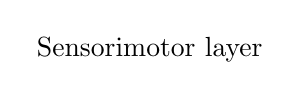
\begin{tikzpicture}
        \node at (0,0) (sensori) {Sensorimotor layer};
        %\node [subpart, below=0.2 of sensori.south west, anchor=north west, align=left] (perception) {{\bf Perception} \\ 2D markers, RGB-D, motion capture};
        %\node [subpart, align=right, right=0.2 of perception] {{\bf Actuation} \\ Head's pan-tilt unit, grippers, arms, wheels};
      \end{tikzpicture}
  };

  %%% Separation between deliberative layer and sensori-motor layer
  \draw[dotted, thick] (-8,-5) -- (12, -5);

  %%% Relations between components
  \path (shary.340) edge [<->, bend left] node[label] {motion plan \\ requests} (mhp);
  \path (shary.west) edge [<->, bend right] node[label] {shared \\ plans} (hatp);
  \path (hatp) edge [<->, bend right] node[label] (domain) {world model and \\ agents beliefs} (oro.170);
  \path (dialogs) edge [<->, bend left] node[label] (nlp) {natural language \\ grounding} (oro.190);
  \path (spark.100) edge [->, bend right] node[label] (symfact) {symbolic \\ facts} (oro);
  \path (spark.5) edge [->, bend right] node[label] {environment\\model} (mhp);
  \path (shary) edge [<->, bend left] node[label] (evts) {events, \\ world model and \\ agents beliefs} (oro);
  \path (shary) edge [<->, bend left] node[label] {action monitoring \\ and management of \\ position hypotheses} (spark);
  \path (lowlevel) edge [->] (spark);
  \path (lowlevel.east) edge [<-, bend right=80, looseness=1.5] node[label] {atomic\\actions} (shary.east);

  \only<2>{
      \fill[fill opacity=.7,white] (current bounding box.north west) rectangle (current bounding box.south east);
      \node[stmt] at (symfact) {isOn(bottle, table)\\lookAt(human1, bottle)};
      \node[stmt] at (nlp) {lookAt(human1, ?obj)\\desires(human1, PickUp, bottle)};
      \node[stmt] at (domain) {isAvailable(?gripper) $\wedge$ isA(?gripper, Gripper)\\isOn(bottle, ?obj)};
      \node[stmt] at (evts) {isA(action23425, PickUp) $\wedge$ currentlyPerforming(action23425)};
  }
\end{tikzpicture}
}
\begin{flushright}
\scriptsize -- based on \cite{lemaignan2012towards}
\end{flushright}
\end{frame}

\begin{frame}{...pick up your options!}

    \begin{itemize}
        \item Internal simulation (HAMMER)
        \item Mental Imagery (SOAR), Pre-supposition accommodation (GSM)
        \item Emotion recognition/generation
        \item ...
    \end{itemize}
\end{frame}


\begin{frame}{Highlights}

    \begin{itemize}
        \item {\Medium well-established theoretical grounds} in formal logics
        \item {\Medium explicit}, {\Medium high-level semantics} (good for NLP for instance!)
        \item good engineering properties (modular, loose coupling,...)
        \item $\Rightarrow$ {\Medium close to the human level} (both for the users and the developers)
    \end{itemize}
    
    \only<2>{

    \begin{itemize}
        \item {\Medium very successful} so far
        \item {\Medium fundamentally top-down} approach $\Rightarrow$ somewhat difficult to match with
            the constructive approach of developmental psychology
        \item {\Medium learning} is an {\Medium after-thought}
        \item representation of {\Medium uncertainty not natural}
        \item {\Medium hard to deal with time} (chronicles, fluents,...?)
    \end{itemize}
    }


\end{frame}

\begin{frame}{Sub-symbolic architectures}

    \begin{itemize}
        \item<1-> {\Medium (Hierarchical) Self-Organizing
            Maps}~\cite{morse2010epigenetic}
        \item<2-> {\Medium Memory network}~\cite{baxter2013cognitive}
        \refToContrib{Paul's contribution}
    \end{itemize}

    \centering
    \only<1>{

        \resizebox{0.7\linewidth}{!}{%

        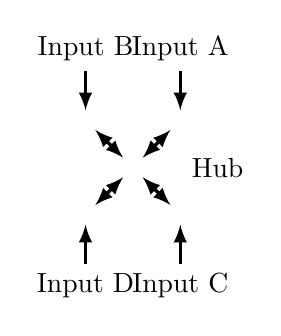
\begin{tikzpicture}[
                >=latex,
                node distance=0.5,
                every edge/.style={draw, very thick},
                every node/.style={font=\Medium}
            ]

            \node (hub) {\usebox{\som}};
            \node[above right=of hub] (somA) {\usebox{\som}};
            \node[above left=of hub] (somB) {\usebox{\som}};
            \node[below right=of hub] (somC) {\usebox{\som}};
            \node[below left=of hub] (somD) {\usebox{\som}};

            \node[above=of somA] (labA) {Input A};
            \node[above=of somB] (labB) {Input B};
            \node[below=of somC] (labC) {Input C};
            \node[below=of somD] (labD) {Input D};
            \node[right=of hub] (labHub) {Hub};

            \path (labA) edge [->] (somA);
            \path (labB) edge [->] (somB);
            \path (labC) edge [->] (somC);
            \path (labD) edge [->] (somD);

            \path (hub) edge [<->] (somA);
            \path (hub) edge [<->] (somB);
            \path (hub) edge [<->] (somC);
            \path (hub) edge [<->] (somD);

        \end{tikzpicture}%
    }

    }
    \only<2>{
        \resizebox{0.7\linewidth}{!}{%
        \begin{tikzpicture}[
                >=latex,
                every edge/.style={draw, very thick},
                every node/.style={font=\Medium,align=center},
                input/.style={draw,circle, inner sep=0pt,minimum size=0.6cm}
            ]

            % draw the units
            \foreach \x [count=\xi] in {0, 120, 240}
                \foreach \y [count=\yi] in {-.6, 0, .6}
                    %\node[input, ball color=orange!\x!blue] at ($(\x:3)!\y!90:(0,0)$) (i\xi\yi) {};
                    \node[input, fill=hriSec3Comp!\x!hriSec1Comp] at ($(\x:3)!\y!90:(0,0)$) (i\xi\yi) {};

            \node[draw,rounded corners, fit=(i11)(i12)(i13)] (modA) {};
            \node[draw,rounded corners, rotate fit=120,fit=(i21)(i22)(i23)] (modB) {};
            \node[draw,rounded corners, rotate fit=60,fit=(i31)(i32)(i33)] (modC) {};

            \node at (180:5.5) {Modalities} edge[->] (modB) edge[->] (modC);
            \node at (-40:6) {Input\\units} edge[->] (i13) edge[->] (i31);

            \path[draw,dashed, hriSec3Dark, thick]  (i23) -- (i11) -- (i31) -- (i23);
            \path[draw,dotted, hriSec3Dark, thick] (i23) -- (i12) -- (i32) -- (i23);
            \path[draw, hriSec3Dark] (i21) -- (i13) -- (i33) -- (i21);

            \node at (1,1) {Associative\\links};
        \end{tikzpicture}
    }
    }

\end{frame}

\imageframe[black]{}{era}

\begin{frame}{Highlights}
    \begin{itemize}
        \item often {\Medium general principled approaches}
        \item {\Medium learning} is intrinsic and fundamental
        \item {\Medium emergent features} (eg concept priming)
    \end{itemize}
    \only<2>{
    \begin{itemize}
        %\item principled approach brings {\Medium predictive power}
        \item more directly comparable to human cognitive appartus
        \item applications to high-level socio-cognitive tasks only emerging
        \item {\Medium still hard to deal with time!}
    \end{itemize}
}
\end{frame}

\begin{frame}{Hybrid architectures}

    \only<1>{What about...}
    \only<3>{or...}
    \only<5>{or even...}
    \only<2,4,6>{
\resizebox{\paperwidth}{!}{%

\tikzset{subpart/.style={draw, font=\scriptsize, fill opacity=0.5, text opacity=1, fill=white!50}}
\begin{tikzpicture}[
    >=latex,
    every edge/.style={draw, very thick},
    skill/.style={draw, rounded corners, align=center, inner sep=5pt, fill=black!20},
    stmt/.style={align=center, font=\Medium},
    label/.style={midway, align=center, font=\scriptsize, fill=white}]

  %%% ORO
    \only<2>{
        \node at (0,0)[skill, ultra thick, fill=hriSec2Dark!50] (oro) {{\Medium Memory} knowledge base(s)\\ \footnotesize typically a symbolic blackboard};
    }
    \only<4,6>{
    \node at (0,0)[skill, ultra thick, fill=hriSec2Dark!50] (oro) {
            \resizebox{0.4\linewidth}{!}{%
        \begin{tikzpicture}[
                >=latex,
                every edge/.style={draw, very thick},
                every node/.style={font=\Medium,align=center},
                input/.style={draw,circle, inner sep=0pt,minimum size=0.6cm}
            ]

            % draw the units
            \foreach \x [count=\xi] in {0, 120, 240}
                \foreach \y [count=\yi] in {-.6, 0, .6}
                    %\node[input, ball color=orange!\x!blue] at ($(\x:3)!\y!90:(0,0)$) (i\xi\yi) {};
                    \node[input, fill=hriSec3Comp!\x!hriSec1Comp] at ($(\x:3)!\y!90:(0,0)$) (i\xi\yi) {};

            \node[draw,rounded corners, fit=(i11)(i12)(i13)] (modA) {};
            \node[draw,rounded corners, rotate fit=120,fit=(i21)(i22)(i23)] (modB) {};
            \node[draw,rounded corners, rotate fit=60,fit=(i31)(i32)(i33)] (modC) {};

            \path[draw,dashed, hriSec3Dark, thick]  (i23) -- (i11) -- (i31) -- (i23);
            \path[draw,dotted, hriSec3Dark, thick] (i23) -- (i12) -- (i32) -- (i23);
            \path[draw, hriSec3Dark] (i21) -- (i13) -- (i33) -- (i21);

            \node at (1,1) {Associative\\links};
        \end{tikzpicture}
    }

    };
  }

  %%% HATP
    \node at (-6, 2.5)[skill, fill=hriSec1!50] (hatp) {{\Medium Task planner}\\ \footnotesize ideally human-aware};
  
  %%% DIALOGS
    \node at (-6, -3) [skill, fill=hriSec3Dark!50] (dialogs) {{\Medium Multi-modal
    communication}\\NLP, back-channel,...};

  %%% SPARK
  \node at (4,-4)[skill, fill=hriSec3!50] (spark) {%
      \begin{tikzpicture}
          \node at (0,0) (geom) {{\Medium Situation Assessment} -- geometric \& temporal reasoning};
        \node [subpart, below=0.2 of geom.south west, anchor=north west] (world-update) {Sensors fusion};
        \node [subpart, right=0.2 of world-update] (geom-model) {Geometric model of the environment};
        \node [subpart, right=0.2 of geom-model] (fact-prod) {Symbolic facts production};
      \end{tikzpicture}
    };

  %%% MHP
    \node at (9,0)[skill, fill=hriSec3CompDark!50] (mhp) {Motion and manipulation \\ planning};

  %%% SHARY
  \node at (4,4.5)[skill, fill=hriSec1Comp!50] (shary) {%
      \begin{tikzpicture}
        \node at (0,0) (exec) {\Medium Execution Controller};
        \node [subpart, below=0.2 of exec.south west, anchor=north west] (plans) {Goal \& Plans \\ management};
        \node [subpart, right=0.2 of plans] (sit-asses) {Situation assessment \\ and context management};
        \node [subpart, right=0.2 of sit-asses] {Action instantiation, \\ execution and monitoring};
      \end{tikzpicture}
    };


  %%% LOWLEVEL
\only<2,6>{
    \node [skill, below=0.7 of spark] (lowlevel1) {\usebox{\som}};
    \node [skill, left=of lowlevel1] (lowlevel2) {\usebox{\som}};
    \node [skill, right=of lowlevel1] (lowlevel) {\usebox{\som}};

}
\only<4>{
  \node [skill, below=0.7 of spark] (lowlevel) {%
      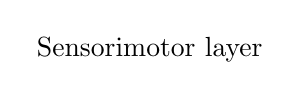
\begin{tikzpicture}
        \node at (0,0) (sensori) {Sensorimotor layer};
        %\node [subpart, below=0.2 of sensori.south west, anchor=north west, align=left] (perception) {{\bf Perception} \\ 2D markers, RGB-D, motion capture};
        %\node [subpart, align=right, right=0.2 of perception] {{\bf Actuation} \\ Head's pan-tilt unit, grippers, arms, wheels};
      \end{tikzpicture}
  };
  }

  %%% Separation between deliberative layer and sensori-motor layer
  \draw[dotted, thick] (-8,-5.5) -- (12, -5.5);

  %%% Relations between components
  \path (shary.340) edge [<->, bend left] (mhp);
  \path (shary.west) edge [<->, bend right] (hatp);
  \path (hatp) edge [<->, bend right] (oro.170);
  \path (dialogs) edge [<->, bend left] (oro.190);
  \path (spark.100) edge [->, bend right] (oro);
  \path (spark.5) edge [->, bend right] (mhp);
  \path (shary) edge [<->, bend left] (oro);
  \path (shary) edge [<->, bend left] (spark);
  \path (lowlevel) edge [->] (spark);
  \only<2,6>{
  \path (lowlevel1) edge [->] (spark);
  \path (lowlevel2) edge [->] (spark);
  }
  \path (lowlevel.east) edge [<-, bend right=80, looseness=1.5] (shary.east);

\end{tikzpicture}
}
}


\end{frame}

\begin{frame}{Hybrid architectures: epistemic arguments}

    The {\Medium computational functionalism} argument~\cite{vernon2014artifical}:
    \begin{quote}
        \doublequoted{the physical realization of the computational model is inconsequential to the model}
    \end{quote}

    \uncover<2>{
        Embodied cognition takes the opposite view.\par
        
        Some see the symbolic/sub-symbolic questions as an instantiation of this argument.
    }

\end{frame}

\begin{frame}{Cross-disciplinary ``Impedance Matching''}

    The choice of a computational model impacts how {\Medium legible} the architecture is
    to other disciplines:

    \begin{itemize}
        \item {\Medium psycholinguistics} will be more comfortable manipulating
            symbolic architectures;
        \item {\Medium neurosciences} may be more comfortable with certain
            sub-symbolic approaches (but not all of them: deep learning 
            is hardly a biologically inspired neural technique)
    \end{itemize}
    
    {\Medium $\Rightarrow$ ``epistemic impedance''}

    \only<2>{
        Some disciplines are however mostly {\Medium agnostic}\\
        cognitive psy., developmental psy.,...
    }

    \only<3>{
        Also relevant is the nature of {\Medium predictions} you want to
        generate or test (eg, reaction time vs language competencies).
    }


\end{frame}

\begin{frame}{A few internal cognitive functions}

    \begin{table}[]
        \begin{tabularx}{\linewidth}{lp{4.5cm}p{4.5cm}}
            \toprule
                     & {\Medium Symbolic}  & {\Medium Sub-symbolic}\\
            \midrule
            {\Medium Concepts} & taxonomies, \newline external knowledge integration & conceptualization \\
            {\Medium Memory}   & facts storage & associative memory,\newline priming \\
            {\Medium Planning}   & Plenty\newline (prototypically: HTN) & recurrent
            networks~\cite{rueckert2016recurrent} \\
            ... & & \\
            \bottomrule
        \end{tabularx}
        \label{tab:options}
    \end{table}
\end{frame}

\begin{frame}{Side-to-side}

    \scriptsize
    \begin{multicols}{2}

        \centering{\Medium Symbolic}

    \begin{itemize}
        \item {\Medium well-established theoretical grounds} in formal logics
        \item {\Medium explicit}, {\Medium high-level semantics}
        \item good engineering properties (modular, loose coupling,...)
        \item $\Rightarrow$ {\Medium close to the human level} (both for the users and the developers)
        \item {\Medium very successful} so far
        \item {\Medium fundamentally top-down} approach $\Rightarrow$ somewhat difficult to match with
            the constructive approach of developmental psychology
        \item {\Medium learning} is an {\Medium after-thought}
        \item representation of {\Medium uncertainty not natural}
        \item {\Medium hard to deal with time} (chronicles, fluents,...?)
    \end{itemize}

    \columnbreak

    \centering{\Medium Sub-symbolic}

    \begin{itemize}
        \item often {\Medium principled approaches}
        \item {\Medium learning} is intrinsic and fundamental
        \item {\Medium interesting features} come for free (eg concept priming)
        \item principled approach brings {\Medium predictive power}
        \item applications to high-level socio-cognitive tasks only emerging
        \item {\Medium still hard to deal with time!}
    \end{itemize}

    \end{multicols}
\end{frame}

\begin{frame}{Discussion directions}

    \begin{itemize}

    \item Does sHRI shed a particular light on the question?
    \item Does {\Medium hybrid architecture} means ``a bit of
        both with bridges in the middle'', or may it be an independent principled
        model?
    \item Should we attempt to bridge? $\Rightarrow$ CogArch as a methodology!

    \end{itemize}

    35 minutes of open discussion, plus one presentation

\end{frame}

\begin{frame}{Bibliography}
\begin{thebibliography}{10}
\footnotesize
    \beamertemplatearticlebibitems
    \bibitem{baxter2013cognitive}
    P. Baxter, J. de Greeff, T. Belpaeme
    \newblock \doublequoted{Cognitive Architecture for HRI: Towards behavioural
    alignment}
    \newblock 2013


    \beamertemplatearticlebibitems
    \bibitem{lemaignan2012towards}
    S. Lemaignan, R. Alami, A. K. Pandey, M. Warnier, J. Guitton
    \newblock \doublequoted{Towards Grounding Human-Robot Interaction}
    \newblock 2012

    \beamertemplatearticlebibitems
    \bibitem{morse2010epigenetic}
    A. Morse, J. de Greeff, T. Belpaeme, A. Cangelosi
    \newblock \doublequoted{Epigenetic Robotics Architecture}
    \newblock 2010

    \beamertemplatearticlebibitems
    \bibitem{rueckert2016recurrent}
    A. Rueckert, D. Kappel, D. Tanneberg, D. Pecevski, J. Peters
    \newblock \doublequoted{Recurrent Spiking Networks Solve Planning Tasks}
    \newblock 2016


    \beamertemplatebookbibitems
    \bibitem{vernon2014artifical}
    D. Vernon
    \newblock \doublequoted{Artificial Cognitive Systems}
    \newblock 2013


  \end{thebibliography}
\end{frame}

\end{document}






